\section{lemma7}
\begin{lemma}
\end{lemma}

Suppose we have a Riemann sphere $C$ and a diagram $(C,\iota, \xi)$ and a regular cell complex refinement $\overline{(C,\iota, \xi)}$ and a sheaf $\mathfrak{F}$ singular supported on it such that when restricted to a small disk $D\subset C$, the refinement is a the following figure where two dimensional strata are labeld by tuples.

\begin{figure}[H] % Optional: [h] means here, [t] for top, [b] for bottom, [p] for page of floats
    \centering
    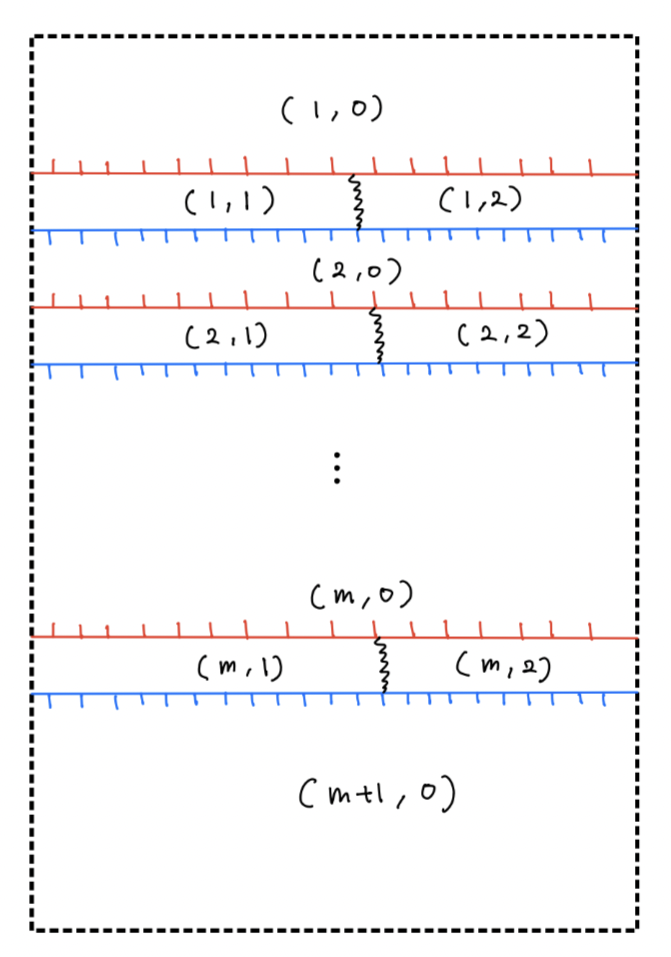
\includegraphics[width=\linewidth]{diagrams/lemma7/1.png} % Adjust the width as needed
    \caption{Your caption here}
    \label{fig:your-label}
\end{figure}

Stalks : \\
$(i,0)$ : $0$\\
$(i,1),(i,2))$ : $\mathbb{C}$\\

Generization maps :\\
$(i,1)\rightarrow (i,2)$ :  multiplication by $a_i \in \mathbb{C}$\\
All the other maps are zero maps.\\

Now we will define isotopy starting from the above sheaf $\mathfrak{F}$ inductively on the number of blue strands(=the number of red strands) so that the final sheaf $\mathfrak{F}'$ is :

\begin{figure}[H] % Optional: [h] means here, [t] for top, [b] for bottom, [p] for page of floats
    \centering
    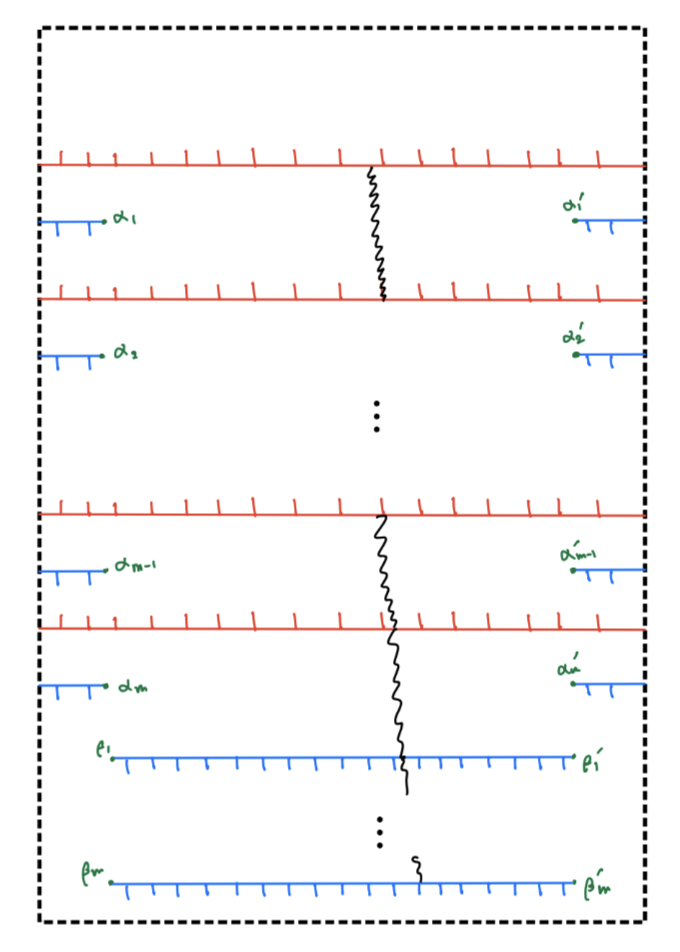
\includegraphics[width=\linewidth]{diagrams/lemma7/2.png} % Adjust the width as needed
    \caption{Your caption here}
    \label{fig:your-label}
\end{figure}


In the above diagram, I have intentionally omitted lines connecting \\
- $\alpha_i$ and $\beta_i$ for $i=1,\cdots,m$\\
- $\alpha'_i$ and $\beta'_i$ for $i=1,\cdots,m$\\
so as not to make diagram too messy. These omitted lines are mutually disjoint and crosses each red strand at most once. Let the crossing of $\overline{\alpha_j \beta_j}$ with the $i^th$ red strand be called $c_{i,j}$ and $\overline{\alpha'_j \beta'_j}$ with the $i^th$ red strand be called $c'_{i,j}$.\\
Let's denote the north, east, west, south of the crossing $c_{i,j}$($c_{i,j}$ resp.) as $N_i,E_i,W_i,S_i$($N'_i,E'_i,W'_i,S'_i$).\\

\bigskip

The final sheaf will be described as follows :\\

Stalks :\\
for $i>j$,\\
- $E_{i,j}$ : $\mathbb{C}^{i-j}$\\
- $S_{i,j}$ : $\mathbb{C}^{i-j-1}$\\
- $W_{i,j}$ : $\mathbb{C}^{i-j}$\\
- $N_{i,j}$ : $\mathbb{C}^{i-j+1}$\\
\\
- $E'_{i,j}$ : $\mathbb{C}^{i-j}$\\
- $S'_{i,j}$ : $\mathbb{C}^{i-j-1}$\\
- $W'_{i,j}$ : $\mathbb{C}^{i-j}$\\
- $N'_{i,j}$ : $\mathbb{C}^{i-j+1}$\\
\\
Generization maps : \\
- maps crossing the blue strands are $\iota_l$.\\
- maps crossing the red strands are $\iota_f$.\\
- maps crossing the squiggly lines :\\
	- for $i\geq 2$, $W_{i,1}\rightarrow E'_{i,1}$ : $T_{1,i-1}$\\
	- $N_{m,1}\rightarrow N'_{m,1}$ : $T_{1,m}$\\
	- $E_{m,j}\rightarrow W'_{m,j}$ : $T_{j+1,m}$\\
	where $T = diag(a_1,\cdots,a_m)$\\
	
Now let's define an isotopy from $\mathfrak{F}$ to $\mathfrak{F}'$ which we call$isotopy_7$.\\
If $n=1$, $isotopy_7$ is a null move.\\
Suppose we have defined $isotopy_7$ upto the number of blue strands(= the number of red strands) less than $m$. Now we define $isotopy_7$ for the number of blue strands(= the number of red strands) equals $m$ :\\

(step1) Apply $isotopy_7$ for the number of blue strands(= the number of red strands) equals $m-1$ on the disk surrounded by purple dotted line which is well-defined by the induction hypothesis.

\begin{figure}[H] % Optional: [h] means here, [t] for top, [b] for bottom, [p] for page of floats
    \centering
    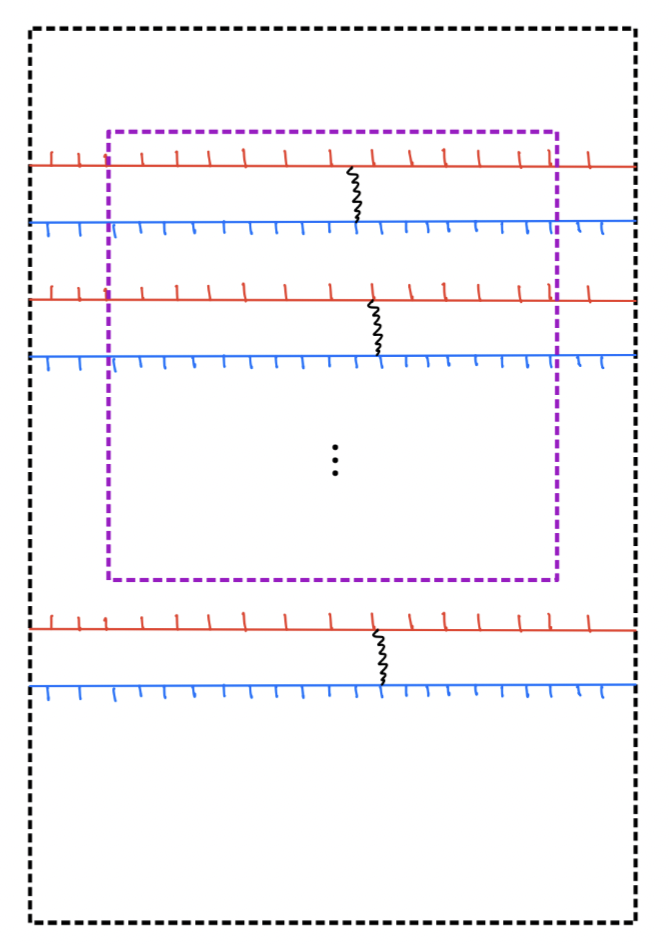
\includegraphics[width=\linewidth]{diagrams/lemma7/3.png} % Adjust the width as needed
    \caption{Your caption here}
    \label{fig:your-label}
\end{figure}

We get the following diagram :

\begin{figure}[H] % Optional: [h] means here, [t] for top, [b] for bottom, [p] for page of floats
    \centering
    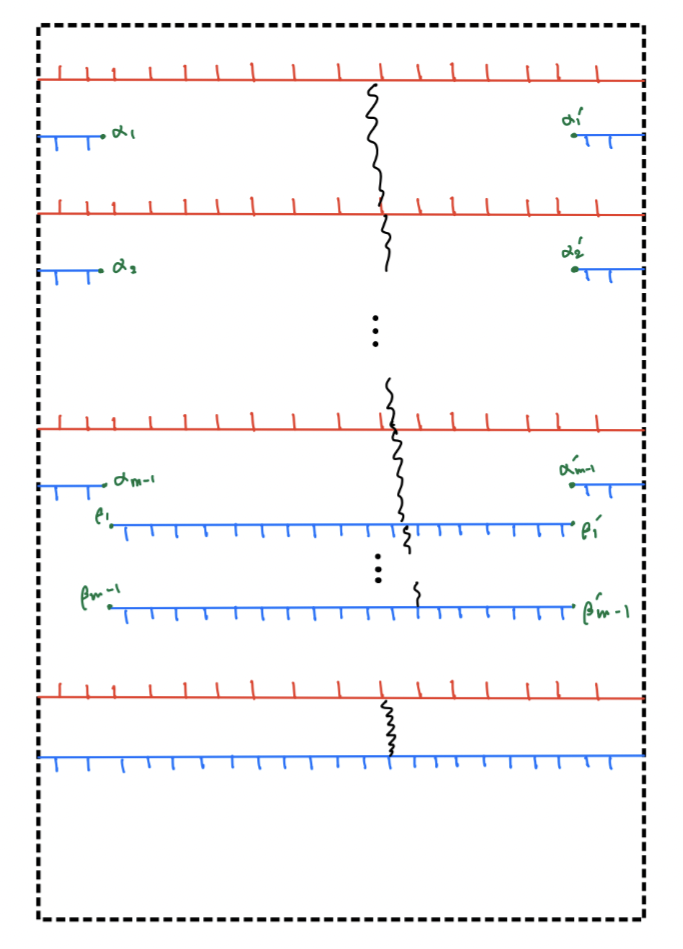
\includegraphics[width=\linewidth]{diagrams/lemma7/4.png} % Adjust the width as needed
    \caption{Your caption here}
    \label{fig:your-label}
\end{figure}
    
(step2) Apply $isotopy_6$ on the disk surrounded by purple dotted line.   

\begin{figure}[H] % Optional: [h] means here, [t] for top, [b] for bottom, [p] for page of floats
    \centering
    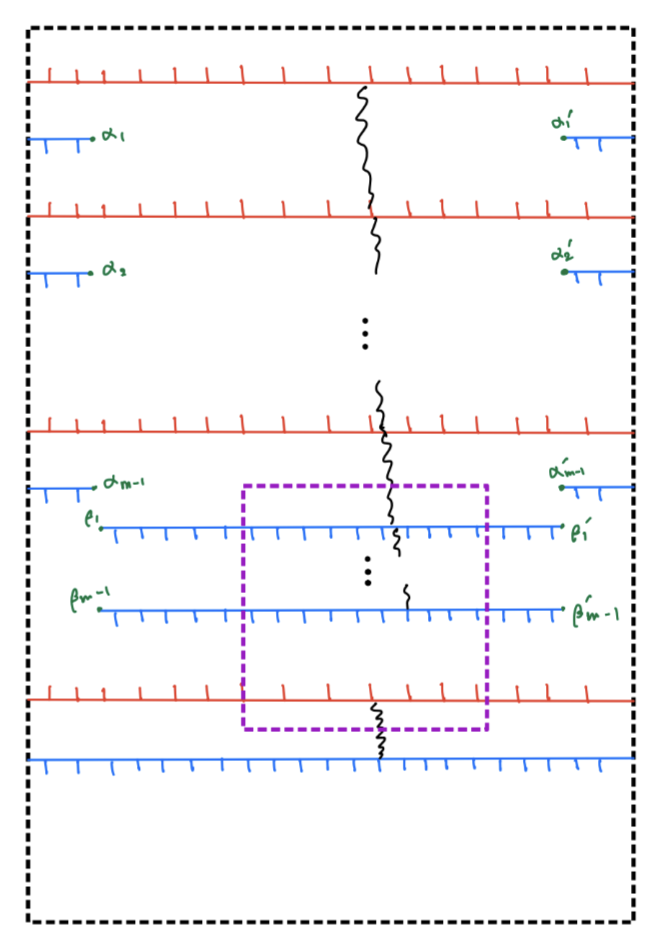
\includegraphics[width=\linewidth]{diagrams/lemma7/5.png} % Adjust the width as needed
    \caption{Your caption here}
    \label{fig:your-label}
\end{figure}

we get the final diagram :

\begin{figure}[H] % Optional: [h] means here, [t] for top, [b] for bottom, [p] for page of floats
    \centering
    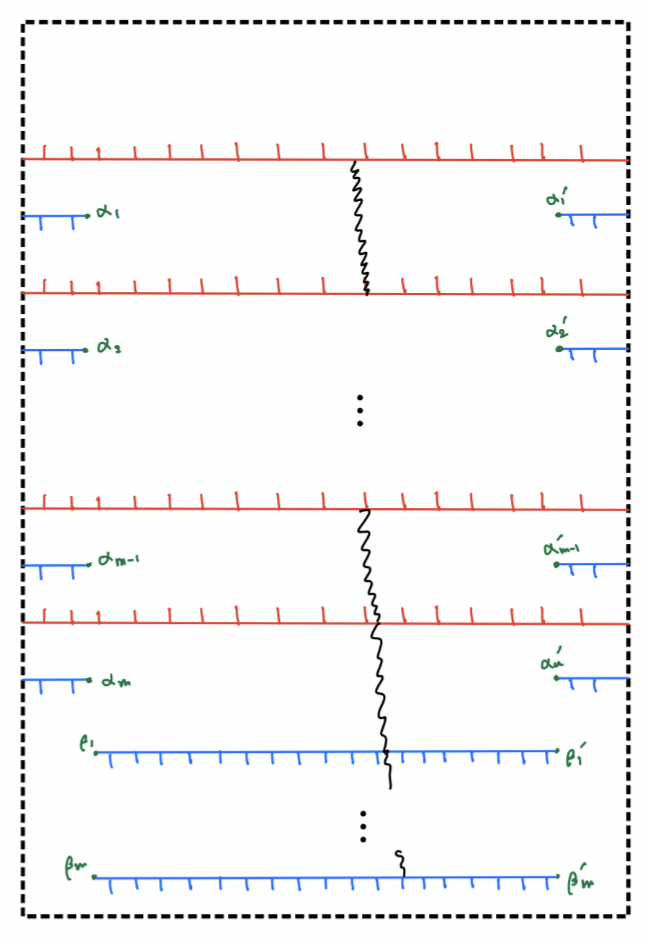
\includegraphics[width=\linewidth]{diagrams/lemma7/6.png} % Adjust the width as needed
    \caption{Your caption here}
    \label{fig:your-label}
\end{figure}